
%% bare_conf.tex
%% V1.3
%% 2007/01/11
%% by Michael Shell
%% See:
%% http://www.michaelshell.org/
%% for current contact information.
%%
%% This is a skeleton file demonstrating the use of IEEEtran.cls
%% (requires IEEEtran.cls version 1.7 or later) with an IEEE conference paper.
%%
%% Support sites:
%% http://www.michaelshell.org/tex/ieeetran/
%% http://www.ctan.org/tex-archive/macros/latex/contrib/IEEEtran/
%% and
%% http://www.ieee.org/

%%*************************************************************************
%% Legal Notice:
%% This code is offered as-is without any warranty either expressed or
%% implied; without even the implied warranty of MERCHANTABILITY or
%% FITNESS FOR A PARTICULAR PURPOSE! 
%% User assumes all risk.
%% In no event shall IEEE or any contributor to this code be liable for
%% any damages or losses, including, but not limited to, incidental,
%% consequential, or any other damages, resulting from the use or misuse
%% of any information contained here.
%%
%% All comments are the opinions of their respective authors and are not
%% necessarily endorsed by the IEEE.
%%
%% This work is distributed under the LaTeX Project Public License (LPPL)
%% ( http://www.latex-project.org/ ) version 1.3, and may be freely used,
%% distributed and modified. A copy of the LPPL, version 1.3, is included
%% in the base LaTeX documentation of all distributions of LaTeX released
%% 2003/12/01 or later.
%% Retain all contribution notices and credits.
%% ** Modified files should be clearly indicated as such, including  **
%% ** renaming them and changing author support contact information. **
%%
%% File list of work: IEEEtran.cls, IEEEtran_HOWTO.pdf, bare_adv.tex,
%%                    bare_conf.tex, bare_jrnl.tex, bare_jrnl_compsoc.tex
%%*************************************************************************

% *** Authors should verify (and, if needed, correct) their LaTeX system  ***
% *** with the testflow diagnostic prior to trusting their LaTeX platform ***
% *** with production work. IEEE's font choices can trigger bugs that do  ***
% *** not appear when using other class files.                            ***
% The testflow support page is at:
% http://www.michaelshell.org/tex/testflow/



% Note that the a4paper option is mainly intended so that authors in
% countries using A4 can easily print to A4 and see how their papers will
% look in print - the typesetting of the document will not typically be
% affected with changes in paper size (but the bottom and side margins will).
% Use the testflow package mentioned above to verify correct handling of
% both paper sizes by the user's LaTeX system.
%
% Also note that the "draftcls" or "draftclsnofoot", not "draft", option
% should be used if it is desired that the figures are to be displayed in
% draft mode.
%
\documentclass[10pt, conference, compsocconf]{IEEEtran}
% Add the compsocconf option for Computer Society conferences.
%
% If IEEEtran.cls has not been installed into the LaTeX system files,
% manually specify the path to it like:
% \documentclass[conference]{../sty/IEEEtran}





% Some very useful LaTeX packages include:
% (uncomment the ones you want to load)


% *** MISC UTILITY PACKAGES ***
%
%\usepackage{ifpdf}
% Heiko Oberdiek's ifpdf.sty is very useful if you need conditional
% compilation based on whether the output is pdf or dvi.
% usage:
% \ifpdf
%   % pdf code
% \else
%   % dvi code
% \fi
% The latest version of ifpdf.sty can be obtained from:
% http://www.ctan.org/tex-archive/macros/latex/contrib/oberdiek/
% Also, note that IEEEtran.cls V1.7 and later provides a builtin
% \ifCLASSINFOpdf conditional that works the same way.
% When switching from latex to pdflatex and vice-versa, the compiler may
% have to be run twice to clear warning/error messages.






% *** CITATION PACKAGES ***
%
%\usepackage{cite}
% cite.sty was written by Donald Arseneau
% V1.6 and later of IEEEtran pre-defines the format of the cite.sty package
% \cite{} output to follow that of IEEE. Loading the cite package will
% result in citation numbers being automatically sorted and properly
% "compressed/ranged". e.g., [1], [9], [2], [7], [5], [6] without using
% cite.sty will become [1], [2], [5]--[7], [9] using cite.sty. cite.sty's
% \cite will automatically add leading space, if needed. Use cite.sty's
% noadjust option (cite.sty V3.8 and later) if you want to turn this off.
% cite.sty is already installed on most LaTeX systems. Be sure and use
% version 4.0 (2003-05-27) and later if using hyperref.sty. cite.sty does
% not currently provide for hyperlinked citations.
% The latest version can be obtained at:
% http://www.ctan.org/tex-archive/macros/latex/contrib/cite/
% The documentation is contained in the cite.sty file itself.






% *** GRAPHICS RELATED PACKAGES ***
%
\ifCLASSINFOpdf
   \usepackage[pdftex]{graphicx}
  % declare the path(s) where your graphic files are
  % \graphicspath{{../pdf/}{../jpeg/}}
  % and their extensions so you won't have to specify these with
  % every instance of \includegraphics
  % \DeclareGraphicsExtensions{.pdf,.jpeg,.png}
\else
  % or other class option (dvipsone, dvipdf, if not using dvips). graphicx
  % will default to the driver specified in the system graphics.cfg if no
  % driver is specified.
  % \usepackage[dvips]{graphicx}
  % declare the path(s) where your graphic files are
  % \graphicspath{{../eps/}}
  % and their extensions so you won't have to specify these with
  % every instance of \includegraphics
  % \DeclareGraphicsExtensions{.eps}
\fi
% graphicx was written by David Carlisle and Sebastian Rahtz. It is
% required if you want graphics, photos, etc. graphicx.sty is already
% installed on most LaTeX systems. The latest version and documentation can
% be obtained at: 
% http://www.ctan.org/tex-archive/macros/latex/required/graphics/
% Another good source of documentation is "Using Imported Graphics in
% LaTeX2e" by Keith Reckdahl which can be found as epslatex.ps or
% epslatex.pdf at: http://www.ctan.org/tex-archive/info/
%
% latex, and pdflatex in dvi mode, support graphics in encapsulated
% postscript (.eps) format. pdflatex in pdf mode supports graphics
% in .pdf, .jpeg, .png and .mps (metapost) formats. Users should ensure
% that all non-photo figures use a vector format (.eps, .pdf, .mps) and
% not a bitmapped formats (.jpeg, .png). IEEE frowns on bitmapped formats
% which can result in "jaggedy"/blurry rendering of lines and letters as
% well as large increases in file sizes.
%
% You can find documentation about the pdfTeX application at:
% http://www.tug.org/applications/pdftex





% *** MATH PACKAGES ***
%
%\usepackage[cmex10]{amsmath}
% A popular package from the American Mathematical Society that provides
% many useful and powerful commands for dealing with mathematics. If using
% it, be sure to load this package with the cmex10 option to ensure that
% only type 1 fonts will utilized at all point sizes. Without this option,
% it is possible that some math symbols, particularly those within
% footnotes, will be rendered in bitmap form which will result in a
% document that can not be IEEE Xplore compliant!
%
% Also, note that the amsmath package sets \interdisplaylinepenalty to 10000
% thus preventing page breaks from occurring within multiline equations. Use:
%\interdisplaylinepenalty=2500
% after loading amsmath to restore such page breaks as IEEEtran.cls normally
% does. amsmath.sty is already installed on most LaTeX systems. The latest
% version and documentation can be obtained at:
% http://www.ctan.org/tex-archive/macros/latex/required/amslatex/math/





% *** SPECIALIZED LIST PACKAGES ***
%
%\usepackage{algorithmic}
% algorithmic.sty was written by Peter Williams and Rogerio Brito.
% This package provides an algorithmic environment fo describing algorithms.
% You can use the algorithmic environment in-text or within a figure
% environment to provide for a floating algorithm. Do NOT use the algorithm
% floating environment provided by algorithm.sty (by the same authors) or
% algorithm2e.sty (by Christophe Fiorio) as IEEE does not use dedicated
% algorithm float types and packages that provide these will not provide
% correct IEEE style captions. The latest version and documentation of
% algorithmic.sty can be obtained at:
% http://www.ctan.org/tex-archive/macros/latex/contrib/algorithms/
% There is also a support site at:
% http://algorithms.berlios.de/index.html
% Also of interest may be the (relatively newer and more customizable)
% algorithmicx.sty package by Szasz Janos:
% http://www.ctan.org/tex-archive/macros/latex/contrib/algorithmicx/




% *** ALIGNMENT PACKAGES ***
%
%\usepackage{array}
% Frank Mittelbach's and David Carlisle's array.sty patches and improves
% the standard LaTeX2e array and tabular environments to provide better
% appearance and additional user controls. As the default LaTeX2e table
% generation code is lacking to the point of almost being broken with
% respect to the quality of the end results, all users are strongly
% advised to use an enhanced (at the very least that provided by array.sty)
% set of table tools. array.sty is already installed on most systems. The
% latest version and documentation can be obtained at:
% http://www.ctan.org/tex-archive/macros/latex/required/tools/


%\usepackage{mdwmath}
%\usepackage{mdwtab}
% Also highly recommended is Mark Wooding's extremely powerful MDW tools,
% especially mdwmath.sty and mdwtab.sty which are used to format equations
% and tables, respectively. The MDWtools set is already installed on most
% LaTeX systems. The lastest version and documentation is available at:
% http://www.ctan.org/tex-archive/macros/latex/contrib/mdwtools/


% IEEEtran contains the IEEEeqnarray family of commands that can be used to
% generate multiline equations as well as matrices, tables, etc., of high
% quality.


%\usepackage{eqparbox}
% Also of notable interest is Scott Pakin's eqparbox package for creating
% (automatically sized) equal width boxes - aka "natural width parboxes".
% Available at:
% http://www.ctan.org/tex-archive/macros/latex/contrib/eqparbox/





% *** SUBFIGURE PACKAGES ***
%\usepackage[tight,footnotesize]{subfigure}
% subfigure.sty was written by Steven Douglas Cochran. This package makes it
% easy to put subfigures in your figures. e.g., "Figure 1a and 1b". For IEEE
% work, it is a good idea to load it with the tight package option to reduce
% the amount of white space around the subfigures. subfigure.sty is already
% installed on most LaTeX systems. The latest version and documentation can
% be obtained at:
% http://www.ctan.org/tex-archive/obsolete/macros/latex/contrib/subfigure/
% subfigure.sty has been superceeded by subfig.sty.



%\usepackage[caption=false]{caption}
%\usepackage[font=footnotesize]{subfig}
% subfig.sty, also written by Steven Douglas Cochran, is the modern
% replacement for subfigure.sty. However, subfig.sty requires and
% automatically loads Axel Sommerfeldt's caption.sty which will override
% IEEEtran.cls handling of captions and this will result in nonIEEE style
% figure/table captions. To prevent this problem, be sure and preload
% caption.sty with its "caption=false" package option. This is will preserve
% IEEEtran.cls handing of captions. Version 1.3 (2005/06/28) and later 
% (recommended due to many improvements over 1.2) of subfig.sty supports
% the caption=false option directly:
%\usepackage[caption=false,font=footnotesize]{subfig}
%
% The latest version and documentation can be obtained at:
% http://www.ctan.org/tex-archive/macros/latex/contrib/subfig/
% The latest version and documentation of caption.sty can be obtained at:
% http://www.ctan.org/tex-archive/macros/latex/contrib/caption/




% *** FLOAT PACKAGES ***
%
%\usepackage{fixltx2e}
% fixltx2e, the successor to the earlier fix2col.sty, was written by
% Frank Mittelbach and David Carlisle. This package corrects a few problems
% in the LaTeX2e kernel, the most notable of which is that in current
% LaTeX2e releases, the ordering of single and double column floats is not
% guaranteed to be preserved. Thus, an unpatched LaTeX2e can allow a
% single column figure to be placed prior to an earlier double column
% figure. The latest version and documentation can be found at:
% http://www.ctan.org/tex-archive/macros/latex/base/



%\usepackage{stfloats}
% stfloats.sty was written by Sigitas Tolusis. This package gives LaTeX2e
% the ability to do double column floats at the bottom of the page as well
% as the top. (e.g., "\begin{figure*}[!b]" is not normally possible in
% LaTeX2e). It also provides a command:
%\fnbelowfloat
% to enable the placement of footnotes below bottom floats (the standard
% LaTeX2e kernel puts them above bottom floats). This is an invasive package
% which rewrites many portions of the LaTeX2e float routines. It may not work
% with other packages that modify the LaTeX2e float routines. The latest
% version and documentation can be obtained at:
% http://www.ctan.org/tex-archive/macros/latex/contrib/sttools/
% Documentation is contained in the stfloats.sty comments as well as in the
% presfull.pdf file. Do not use the stfloats baselinefloat ability as IEEE
% does not allow \baselineskip to stretch. Authors submitting work to the
% IEEE should note that IEEE rarely uses double column equations and
% that authors should try to avoid such use. Do not be tempted to use the
% cuted.sty or midfloat.sty packages (also by Sigitas Tolusis) as IEEE does
% not format its papers in such ways.





% *** PDF, URL AND HYPERLINK PACKAGES ***
%
\usepackage{url}
% url.sty was written by Donald Arseneau. It provides better support for
% handling and breaking URLs. url.sty is already installed on most LaTeX
% systems. The latest version can be obtained at:
% http://www.ctan.org/tex-archive/macros/latex/contrib/misc/
% Read the url.sty source comments for usage information. Basically,
% \url{my_url_here}.





% *** Do not adjust lengths that control margins, column widths, etc. ***
% *** Do not use packages that alter fonts (such as pslatex).         ***
% There should be no need to do such things with IEEEtran.cls V1.6 and later.
% (Unless specifically asked to do so by the journal or conference you plan
% to submit to, of course. )


% correct bad hyphenation here
\hyphenation{op-tical net-works semi-conduc-tor}


\begin{document}
%
% paper title
% can use linebreaks \\ within to get better formatting as desired
\title{AccTrace: Accessibility in Phases of Requirements Engineering, Design and Coding Software}


% author names and affiliations
% use a multiple column layout for up to two different
% affiliations

\author{\IEEEauthorblockN{
Rodrigo Gon{\c{c}}alves de Branco,
Maria Stela Cagnin and 
Debora Maria Barroso Paiva} \IEEEauthorblockA{School of
Computing\\
Federal University of Mato Grosso do Sul - UFMS\\
Campo Grande - MS, Brasil\\
rodrigo.g.branco@gmail.com,istela@gmail.com,dmbpaiva@gmail.com}
}

% conference papers do not typically use \thanks and this command
% is locked out in conference mode. If really needed, such as for
% the acknowledgment of grants, issue a \IEEEoverridecommandlockouts
% after \documentclass

% for over three affiliations, or if they all won't fit within the width
% of the page, use this alternative format:
% 
%\author{\IEEEauthorblockN{Michael Shell\IEEEauthorrefmark{1},
%Homer Simpson\IEEEauthorrefmark{2},
%James Kirk\IEEEauthorrefmark{3}, 
%Montgomery Scott\IEEEauthorrefmark{3} and
%Eldon Tyrell\IEEEauthorrefmark{4}}
%\IEEEauthorblockA{\IEEEauthorrefmark{1}School of Electrical and Computer Engineering\\
%Georgia Institute of Technology,
%Atlanta, Georgia 30332--0250\\ Email: see http://www.michaelshell.org/contact.html}
%\IEEEauthorblockA{\IEEEauthorrefmark{2}Twentieth Century Fox, Springfield, USA\\
%Email: homer@thesimpsons.com}
%\IEEEauthorblockA{\IEEEauthorrefmark{3}Starfleet Academy, San Francisco, California 96678-2391\\
%Telephone: (800) 555--1212, Fax: (888) 555--1212}
%\IEEEauthorblockA{\IEEEauthorrefmark{4}Tyrell Inc., 123 Replicant Street, Los Angeles, California 90210--4321}}




% use for special paper notices
%\IEEEspecialpapernotice{(Invited Paper)}




% make the title area
\maketitle


\begin{abstract}
Providing accessible web products is a challenge. In particular, the implementation of requirements is still 
a problem for many developers who may not have the necessary skills to perform this task, including difficulty 
in interpreting reference documents. This paper presents the AccTrace, a CASE tool (Eclipse plugin) that uses 
an ontology to specify the technical implementation of accessibility and promotes traceability of accessibility 
requirements from conception to the coding phases. This may give the developer useful information for the 
construction of accessible product.


\end{abstract}

\begin{IEEEkeywords}
Accessibility; Requirement Traceability; Software Development
Process; CASE Tool;

\end{IEEEkeywords}


% For peer review papers, you can put extra information on the cover
% page as needed:
% \ifCLASSOPTIONpeerreview
% \begin{center} \bfseries EDICS Category: 3-BBND \end{center}
% \fi
%
% For peerreview papers, this IEEEtran command inserts a page break and
% creates the second title. It will be ignored for other modes.
\IEEEpeerreviewmaketitle



\section{Introduction}

Internet is considered an important mean of communication, dissemination of information and provision of services in the present day. Providing access to this information to a wide variety of devices, with different technologies and specifications has become a challenge. Mainly, people with special needs require  specially developed products that consider particular techniques promoting accessibility.

Building accessible products is not an easy task and this subject is considered in many research \cite{lazar:04,brajnik:06,zeng:05}. There are specific proposals for integrating usability and accessibility to the processes of Software Engineering, however, many designers and developers do not know how to code to make accessible products \cite{1630123,alves:11}.

The use of tools that support professionals in building accessible solutions is very common because they increase productivity and decrease the effort required. These tools are IDEs, frameworks, simulators, validators and CASE tools. However, research shows that the available tools do not support satisfactorily in relation to accessibility \cite{Trewin:2010:ACT:1805986.1806029}.

The situation is more serious because there are several studies on generic requirements traceability \cite{5970169,292398,5485417,6405269} and few studies on the development of accessibility requirements during the development process of web applications \cite{analuizadias:2010}.

This article presents the AccTrace, a CASE tool developed as an
Eclipse plugin to enable the traceability of accessibility requirements
and deliver relevant information to the developer for
construction of an accessible product. The AccTrace contributes to implementation of MTA \cite{maia:10}, a software process
development based on ISO/IEC 12207 that includes accessibility tasks.

During the development of software, the union among requirements, UML models and the new
approach proposed for implementation of accessibility techniques 
to these relationships result in comments in source code, which is recovered in real time detailing the
information described previously.

In this paper we propose a solution to help ensure that the developer can include accessibility attributes
during the analysis, design and implementation of software to enable that development of accessibility requirements
during the process can produce an accessible product.

The paper is organized as follows. In Section 2, we discuss related work. In Section 3, the approach is explained. In Section 4, the implementation is described. In section 5 the proof of concept is presented. Finally, in Section 6 the conclusions are presented.

\subsection{Related Work}

As pointed out by Dias \cite{analuizadias:2010}, many papers have been published about accessibility evaluation of software products. Another issue discussed in the literature is the execution of user testing. We have observed that the theme \textit {accessibility in the software development process}
is still underexplored \cite{maia:10}.

On the other hand, we can find many studies on requirements traceability \cite{5970169,292398,5485417,6405269}
as well as finding studies using 
ontologies for domain mapping in the development process \cite{5223183,6511842,4148940,5362244}. However, we do not find in the literature specific studies on traceability of
accessibility requirements during the process of software development. 
In other words, we have not found studies that could, at the code level, to rescue the information on the traceability of accessibility 
requirements and UML models.


\section{AccTrace: Background Theory}

The AccTrace was based on the a Accessibility Tasks Model (MTA) 
\cite {maia:10}, considering mainly  subprocess 4 (Software Requirements Analysis), subprocess 5
(Software Project) and subprocess 6 (Software Construction). MTA is inserted into ISO/IEC 12207 Development Process (Standard for Information Technology - Process of Software Life Cicle) aiming to assist analyze, design, implement and evaluate accessible software.

Figure \ref{fig:figmagica} presents the MTA subprocesses considering in this work, the traceability schema
at a high level and the inclusion of accessibility requirements.

\begin{figure}[h!]
\centering
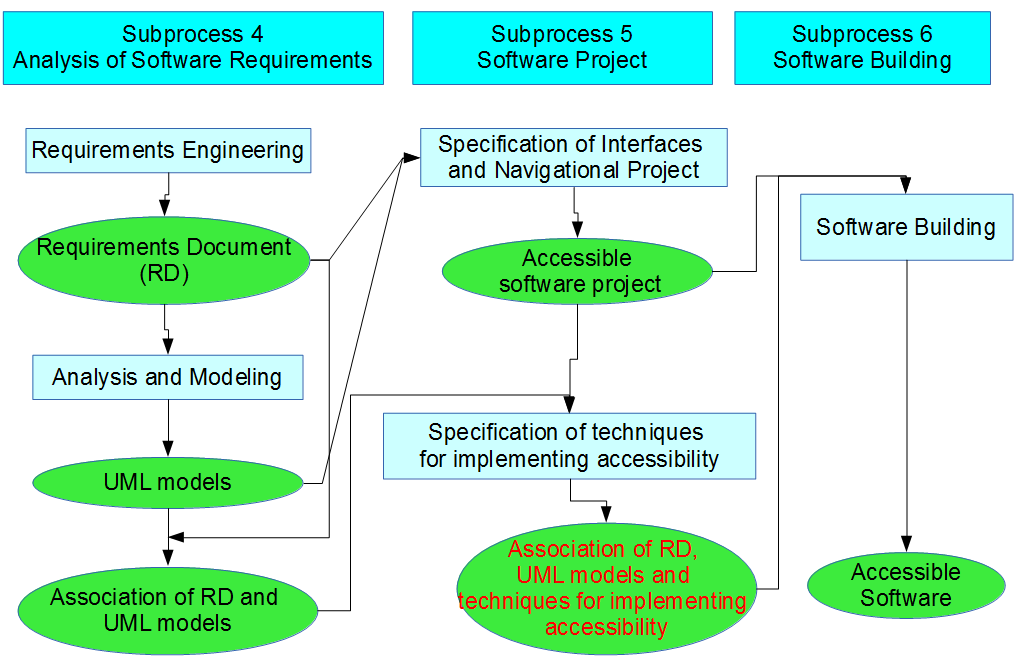
\includegraphics[scale=0.45]{img/figuramagica.png}
\caption{Subprocesses MTA detailing to provide 
accessibility requirements traceability in accordance with the approach adopted in this work}
\label{fig:figmagica}
\end{figure}

The AccTrace assumes that the accessibility specialist is a member of the development team,
having the role of identifying the
accessibility requirements and join requirements,
UML models and implementation techniques for accessibility, as presented following. 


\subsection{Subprocess 4 - Software Requirements Analysis}

The Subprocess 4 brings two accessibility tasks:  (\textbf{Establish and
Documenting the Software Accessibility Requirements } and \textbf{Evaluate
Software Accessibility Requirements}). The output of the task \textbf{Evaluate
Software Accessibility Requirements} generates the artifact \textbf {Requirements Document  
evaluated and approved}.

The construction of UML models in the Modeling and Analysis task, as shown
Figure \ref{fig:figmagica}, receives as input the artifact \textbf{Requirements Document  
evaluated and approved}, so the association of
requirements and models is performed.

\subsection{Subprocess 5 - Software Project}

The Subprocess 5 introduces three accessibility tasks:  (\textbf{Designing
Accessible External Interfaces}, \textbf{Perform Accessible Navigational Project} and 
\textbf {Evaluate Accessibility of Software Project}). The
requirements document and UML models are used to perform
specification of the navigational interfaces project, generating the artifact
\textbf{Accessible Software Project}. At this point, the designer can specify
what are the technical implementation of accessibility and associate them with
requirements and UML models.


\subsection{Subprocess 6 - Software Construction}

The Subprocess 6 has two important tasks for the scope of this work:
(\textbf{Specify Techniques for Implementing Accessibility
at Interface and Code} and \textbf {Code and document each software unit
according to accessibility techniques}). For traceability,
specification of accessibility implementation techniques has been made in
Subprocess 5, missing perform documentation. Step \textbf{Software Construction} (Figure \ref {fig:figmagica}) uses the
artifacts \textbf{Accessible Software Project} and \textbf{Technical Specifications
of Accessibility Implementation} to finally allow the construction of
accessible software.


\section{AccTrace}

In general, the AccTrace implements the traceability mechanism shown in
Figure \ref{fig:figmagica} and, therefore, made use of the following technologies:


\begin{itemize}
  \item Eclipse Juno - IDE;
  \item Requirement Designer v0.8.0 - Requirements Management;
  \item UML Designer v2.1.0 - UML Modeling;
  \item UML to Java Generator v1.0.2 - Code generation;
  \item Java JRE e JDK 1.7 - Plugin development;
  \item Projeto Aegis - ontology mapping accessibility domain (using the WCAG 2.0).
\end{itemize}

Eclipse is a stable platform and was chosen as IDE for several reasons. It
serves as the basis for many products and technologies based on an IDE, providing
an API to facilitate integration. The development of plugins for Eclipse is done directly in the IDE,
in a practical and transparent manner, with much documentation. The language
used for the development of the plugin is Java as well as the code
generated by exportation plugin.

The plugins of requirements management and modeling are developed by Obeo and are interoperable, allowing a smooth integration among the tools. Plugin chosen for generation of code was the UML to Java Generator, developed by
same company. All of these plugins, as well as AccTrace, persist your data as RDF files modeled with EMF format. 
The plugins are available under the Eclipse Public License v1.0 as well as the IDE. Thus, it is possible to study, change and customize their components to achieve the research objectives.

The Aegis Project \cite{aegis:13} defines an ontology for accessibility, described in OWL 1.0 standard, and performs the mapping of concepts of accessibility and scenarios. The available files map the WCAG 2.0 model (including implementation techniques, criteria for success and failure, etc.), screen readers, text browsers, WAI/ARIA, among others.


Figure \ref{fig:association} shows the behavior and relationship of the tools, technologies
and actors involved in the development of AccTrace. Some important information for understanding the figure are presented following:

\begin{figure}[h!]
\centering
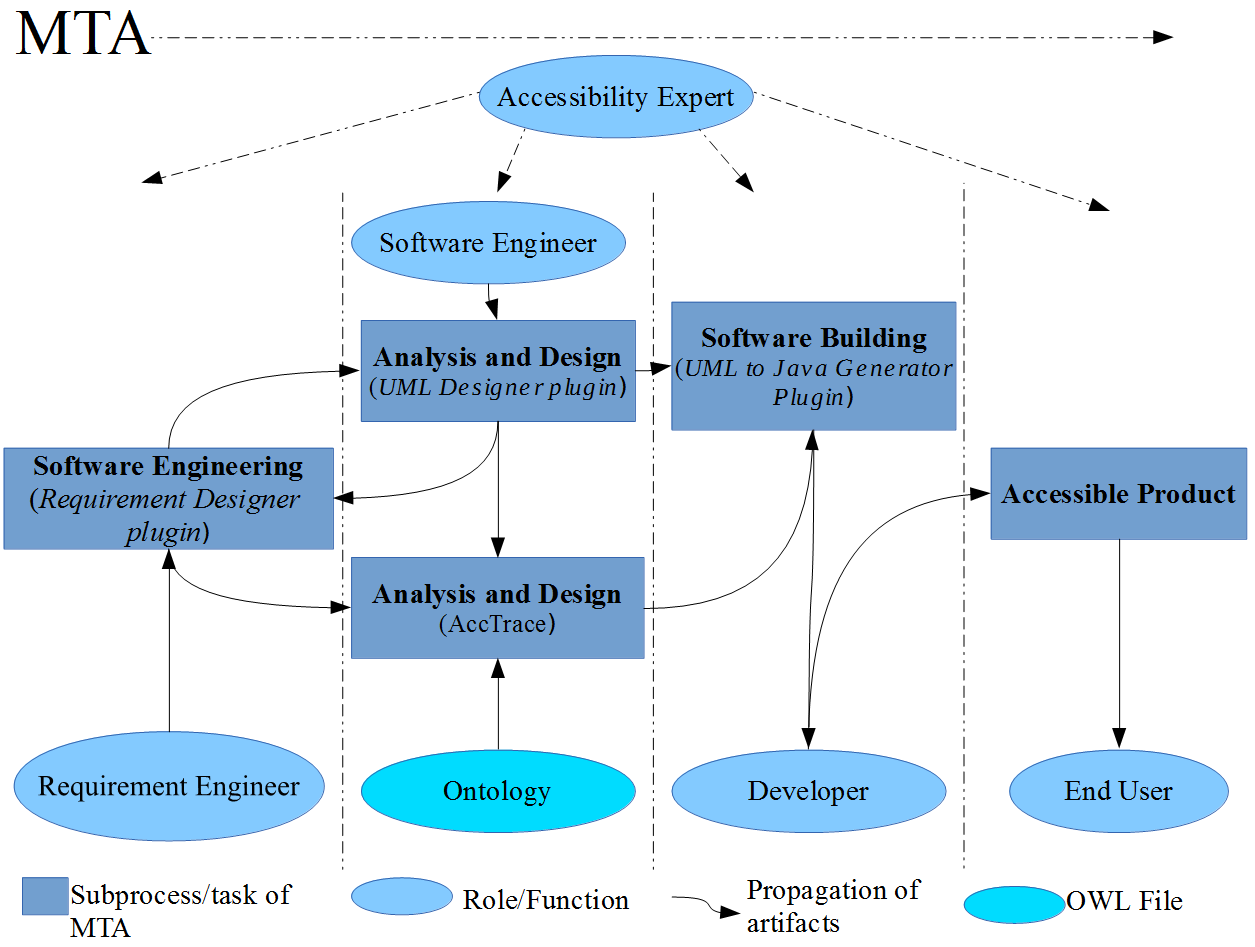
\includegraphics[scale=0.33]{./img/developmentNew2.png}
\caption{Association of tools and actors}
\label{fig:association}
\end{figure}


\begin{itemize}
  \item The MTA is the development process and should cover all phases of this research;
  \item The specialist in accessibility should participate of all development phases
specified in MTA;
  \item Requirements should be collected and reported during the requirements engineering phase
(using  the Requirement Designer tool)and UML models and artifacts
must be generated (using UML Designer tool). The specialist in accessibility should help supply these data, filtering requirements
accessibility so that they are associated with UML models (using the tool Requirement Designer);
  \item The AccTrace retrieves associations and requirements of UML models, allowing the expert to specify the technical implementation of accessibility for each association. Techniques, guidelines, approaches, and others are stored in OWL files embedded in the tool;
    \item The code generation tool produces the stub code from models
UML, adding references to associations of accessibility if necessary;
  \item Developers refine the code until it is ready to become the
accessible product that will be delivered.
\end{itemize}

The tool has three main views in accordance with Figure \ref{fig:acctrace}. 

\begin{figure}[h!]
\centering
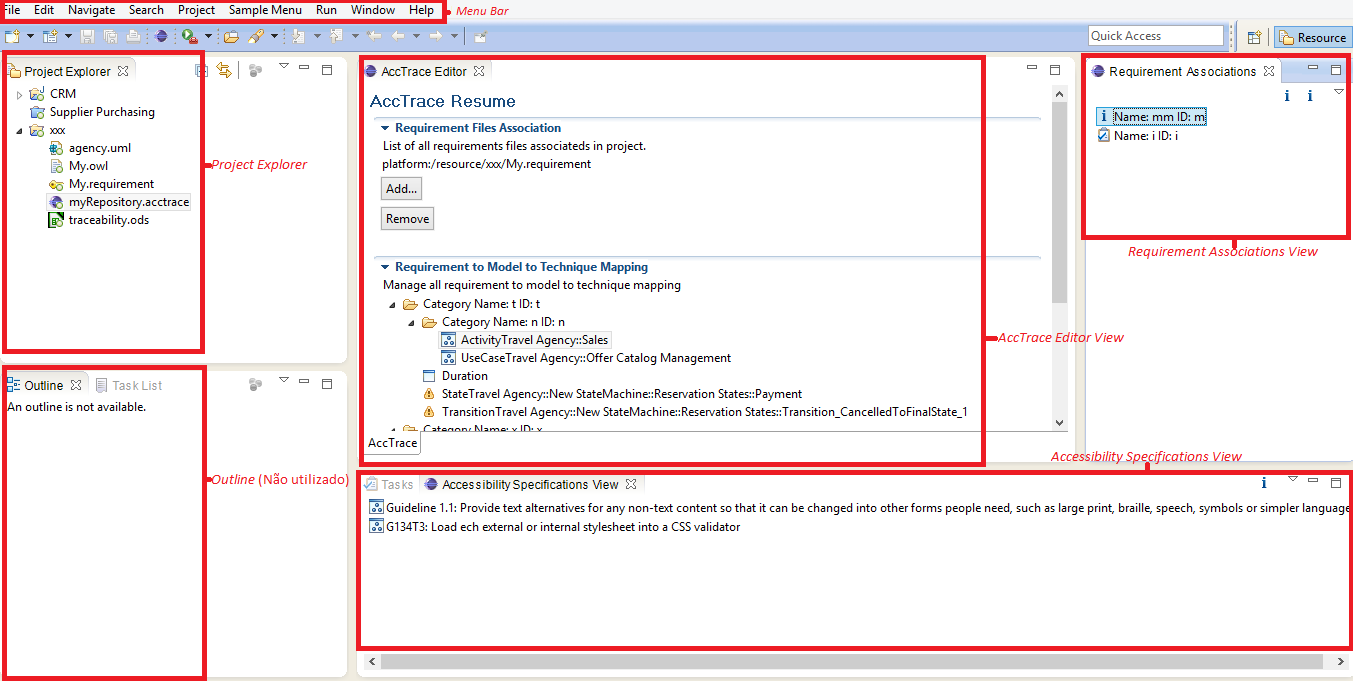
\includegraphics[scale=0.35]{./img/acctrace.png}
\caption{AccTrace plugin in the main screen of
Eclipse IDE}
\label{fig:acctrace}
\end{figure}

In the editor (Editor AccTrace) the designer can change the repositories of requirements and generate associations between UML models, requirements and implementation techniques. in the view requirements (Requirement Associations) he can see which requirements associated
the UML model were selected in the editor. In view of the techniques already linked
(Accessibility Specifications View) he can view the implementation techniques already
associated, according to the UML model selected in the editor and the requirement for accessibility
selected in view of the requirements. The three views are important for the correct functioning
of the plugin.


After selecting the UML model and the requirement, the designer can make the association of
accessibility implementation technique, clicking the right-button mouse on
top of the UML model, as shown in Figure \ref{fig:rightclick}.


\begin{figure}[h!]
\centering
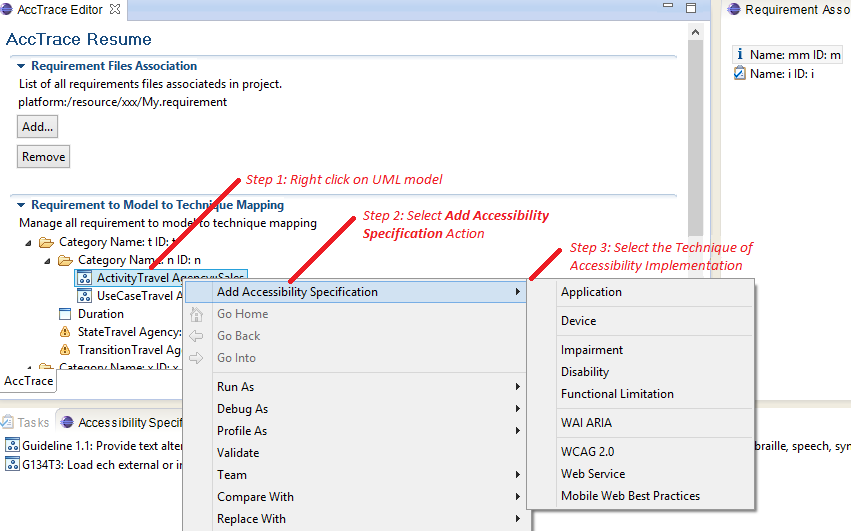
\includegraphics[scale=0.50]{./img/rightclick.png}
\caption{Procedure to make the association of the accessibility implementation technique}
\label{fig:rightclick}
\end{figure}

After the connection between the requirements, UML models and implementation techniques, the designer can generate a traceability matrix.
In this work we used the Apache ODF Toolkit for generating the traceability document with Open-Document Spreadsheet file format (ODS) format. Three worksheets are generated: Requirements \textit {versus} Models, Requirements \textit{versus} Techniques and Templates \textit{versus} techniques. The spreadsheet Requirements \textit{versus} Models list an array of all requirements associated with respective models. Requirements that are not associated with a model are also listed. This situation is expected
just to identify problems that should be corrected. For the Requirements \textit{versus} Techniques and Templates \textit{versus} techniques spreadsheets, only the objects that
are actually referenced in the tool are listed.

Finally, the designer can perform code generation using the UML to Java Generator plugin, which uses the extension point of the Acceleo plugin.
The UML to Java generator plugin was specially modified to recognize the associations between Requirements, UML models and accessibility implementation techniques, creating custom comments in the correct class scopes according to Java regular expression as follows:

\medskip

\noindent
\begin{verbatim}
String regex = "//!ACCTRACE!(/)?([^/\\\\0#]+(/)?)+#([^\\*\\*/])+";
\end{verbatim}
%
\noindent

The regular expression was constructed to allow, through a pre-defined string, recovery of Acctrace file. The personalized 
comment has been designed so as not interfere other
comments language. Started by double slashes (//), it was defined a
identifier that is intended to be unique (! ACCTRACE!), and the ID of the RDF resource has the character ``\#'', which is used to separate 
the resource (file to open) and the element to be gathered (in this case,
association created between the requirement and the UML model). The option of
use a comment line (instead of block comments, for example used by JavaDoc documentation) resulted from the fact
of the comment be included within the body of the class and methods, and case
the programmer decides to comment out the entire code, this may be possible. 

Figure \ref{fig:commentrecovery} shows the steps to retrieve information from a AccTrace comment and Figure \ref{fig:commentview}
shows the view of the retrieved information.


\begin{figure}[h!]
\centering
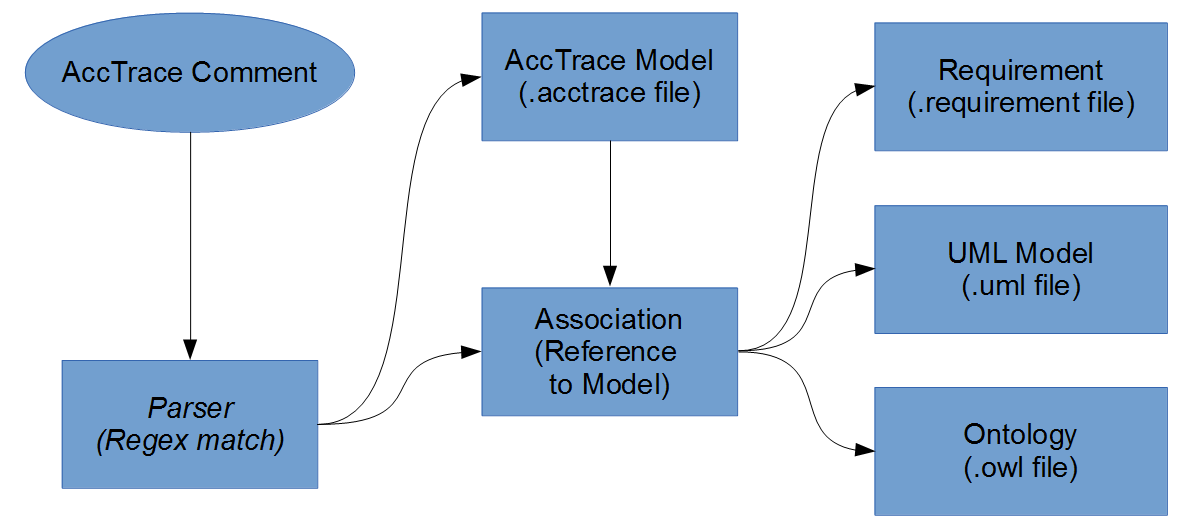
\includegraphics[scale=0.40]{./img/commentrecovery.png}
\caption{Steps to recovery of relevant information through a
default AccTrace comment}
\label{fig:commentrecovery}
\end{figure} 

\begin{figure}[h!]
\centering
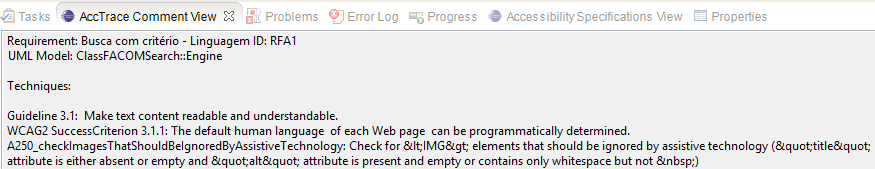
\includegraphics[scale=0.60]{./img/commentview.png}
\caption{Presentation of the selected comment}
\label{fig:commentview}
\end{figure}

\section{Evaluation of the Proposal: Proof of Concept} 

To evalutate the effectiveness of the proposed approach, a software project (web search engine) was created as a proof of concept. Especially, we use the MTA and the AccTrace in this evaluation. The purpose of this proof of concept was to verify if the AccTrace:

\begin{itemize}
  \item Allows the relationship between requirements and use cases with the coding step;
  \item Allows traceability of accessibility requirements, from conception to coding phase;   
  \item Allows the developer can check in code level, the combination of requirements, UML models and implementation techniques of accessibility
\end{itemize}

The objectives listed above have been met:
plugins used are interoperable, allowing the definition and relationship of the requirements and UML models, recovered by step coding tool, traceability could be done in AccTrace plugin and using traceability matrix generated by the tool, the developer manages the from a review AccTrace personalized, and can be retrieved in the coding step by the tool, the traceability could be done in AccTrace plugin. Using traceability matrix generated by the tool, the developer can (from a comment AccTrace personalized) retrieve information about the requirement and associated UML model.

Therefore, it was possible to trace the requirements, from conception and definition, considering the models and UML artifacts,
and finally when it was recovered in the coding phase. The delivery of information that may be useful to the developer is done.
The accessibility expert tells which particular technique accessibility
model / requirement should use as a guide (either approaches, guidelines, success criteria,
techniques, etc.), this information being available by the developer.

The proof of concept demonstrated how user would use the
techniques and tools in a real environment. However, it was not possible to verify
if the steps carried out would actually be used in real project.

The operation of the files built/changed throughout this work was
difficult in some cases. Some difficulties were encountered during proof of concept execution, 
suggesting that some parts of plugin should be improved, so that the usability of
plugin be also improved.



\section{Conclusions}

This study proved to be possible to specify implementation techniques which should
be considered by the developers to promote the accessibility requirements traceability throughout the process. 
The use of an ontology of the Aegis project \cite{aegis:13} was important to achieve this goal, extending the
implementation techniques previously said to approaches, guidelines, success criteria, among others.


We can highlight five major contributions provided by this
work: (a) extend and support the MTA proposed by \cite{maia:10}; (b) address traceability of accessibility requirements in a process
   development that includes accessibility tasks (MTA); (c) allow the specification of implementation techniques of accessibility,
   mapped into a pre-defined ontology; (d) retrieve traceability information through customized comments in the source code and (e) 
provide a tool as a proof of concept.
   

We can indicate how future work: (a) perform a case study with a real project using the MTA and the plugin
   built and customized to promote the generation of traceability and code; (b) study the use of dynamic methods of
   traceability of requirements; (c) perform the mapping of the ontology to other reference
   accessibility models; (d) extend the scope of this work, including suprocesses of tests
   integration of software and the system (subprocesses 7, 8, 9 and 10 of
   MTA);


% trigger a \newpage just before the given reference
% number - used to balance the columns on the last page
% adjust value as needed - may need to be readjusted if
% the document is modified later
%\IEEEtriggeratref{8}
% The "triggered" command can be changed if desired:
%\IEEEtriggercmd{\enlargethispage{-5in}}

% references section

% can use a bibliography generated by BibTeX as a .bbl file
% BibTeX documentation can be easily obtained at:
% http://www.ctan.org/tex-archive/biblio/bibtex/contrib/doc/
% The IEEEtran BibTeX style support page is at:
% http://www.michaelshell.org/tex/ieeetran/bibtex/
\bibliographystyle{IEEEtran}
% argument is your BibTeX string definitions and bibliography database(s)
\bibliography{IEEEabrv,refbibs}
%
% <OR> manually copy in the resultant .bbl file
% set second argument of \begin to the number of references
% (used to reserve space for the reference number labels box)
%\begin{thebibliography}{1}

%\bibitem{IEEEhowto:kopka}
%H.~Kopka and P.~W. Daly, \emph{A Guide to \LaTeX}, 3rd~ed.\hskip 1em plus
%  0.5em minus 0.4em\relax Harlow, England: Addison-Wesley, 1999.

%\end{thebibliography}




% that's all folks
\end{document}


